\documentclass[lang=cn, 11pt, a4paper, cite=authornum, ctexfont]{paper}
\usepackage{siunitx}
\usepackage{pdfpages}
\usepackage{float}
\usepackage{svg}

\title{电子设计实习报告}
\author{卢翼\\21190603}
\institute{南京师范大学\\ 电气与自动化工程学院}
\date{\zhtoday}

\begin{document}

\maketitle

\tableofcontents
\thispagestyle{empty}

\newpage
\setcounter{page}{1}

\section{设计任务和技术指标}

\subsection{设计任务}

\begin{enumerate}
	\item 能用数字显示时、分、秒(23小时59分59秒)。
	\item 具有快速校准时、分的功能。
	\item 具有整点报时功能(从59分51秒开始鸣叫5响,分别为四低一高)。
\end{enumerate}

\subsection{技术指标}

\begin{enumerate}
	\item 产生频率 $f = \SI{1}{\kilo\hertz}$ 的脉冲信号;
	\item 设计分频比为$1000$的分频器,产生$ \SI{1}{\hertz} $的秒脉冲;       
	\item 分别设计60进制计数器和24进制计数器;
	\item 设计用于校时、校分的2选1数据选择器;
	\item 用$\SI{1}{\hertz}$脉冲作为时、分的快速校正信号;
	\item 设计报时电路,前4响$\SI{500}{\hertz}$声音,最后一响$\SI{1}{\kilo\hertz}$。
\end{enumerate}

\subsection{设计工具}

软件: proteus

硬件: 见物料清单

\section{原理框图}

\begin{figure}[H]
	\begin{center}
		\includesvg[width=0.75\textwidth]{svg/原理框图.svg}
		\caption{原理框图}
	\end{center}
\end{figure}

\section{单元电路设计}

\begin{figure}[H]
	\begin{center}
		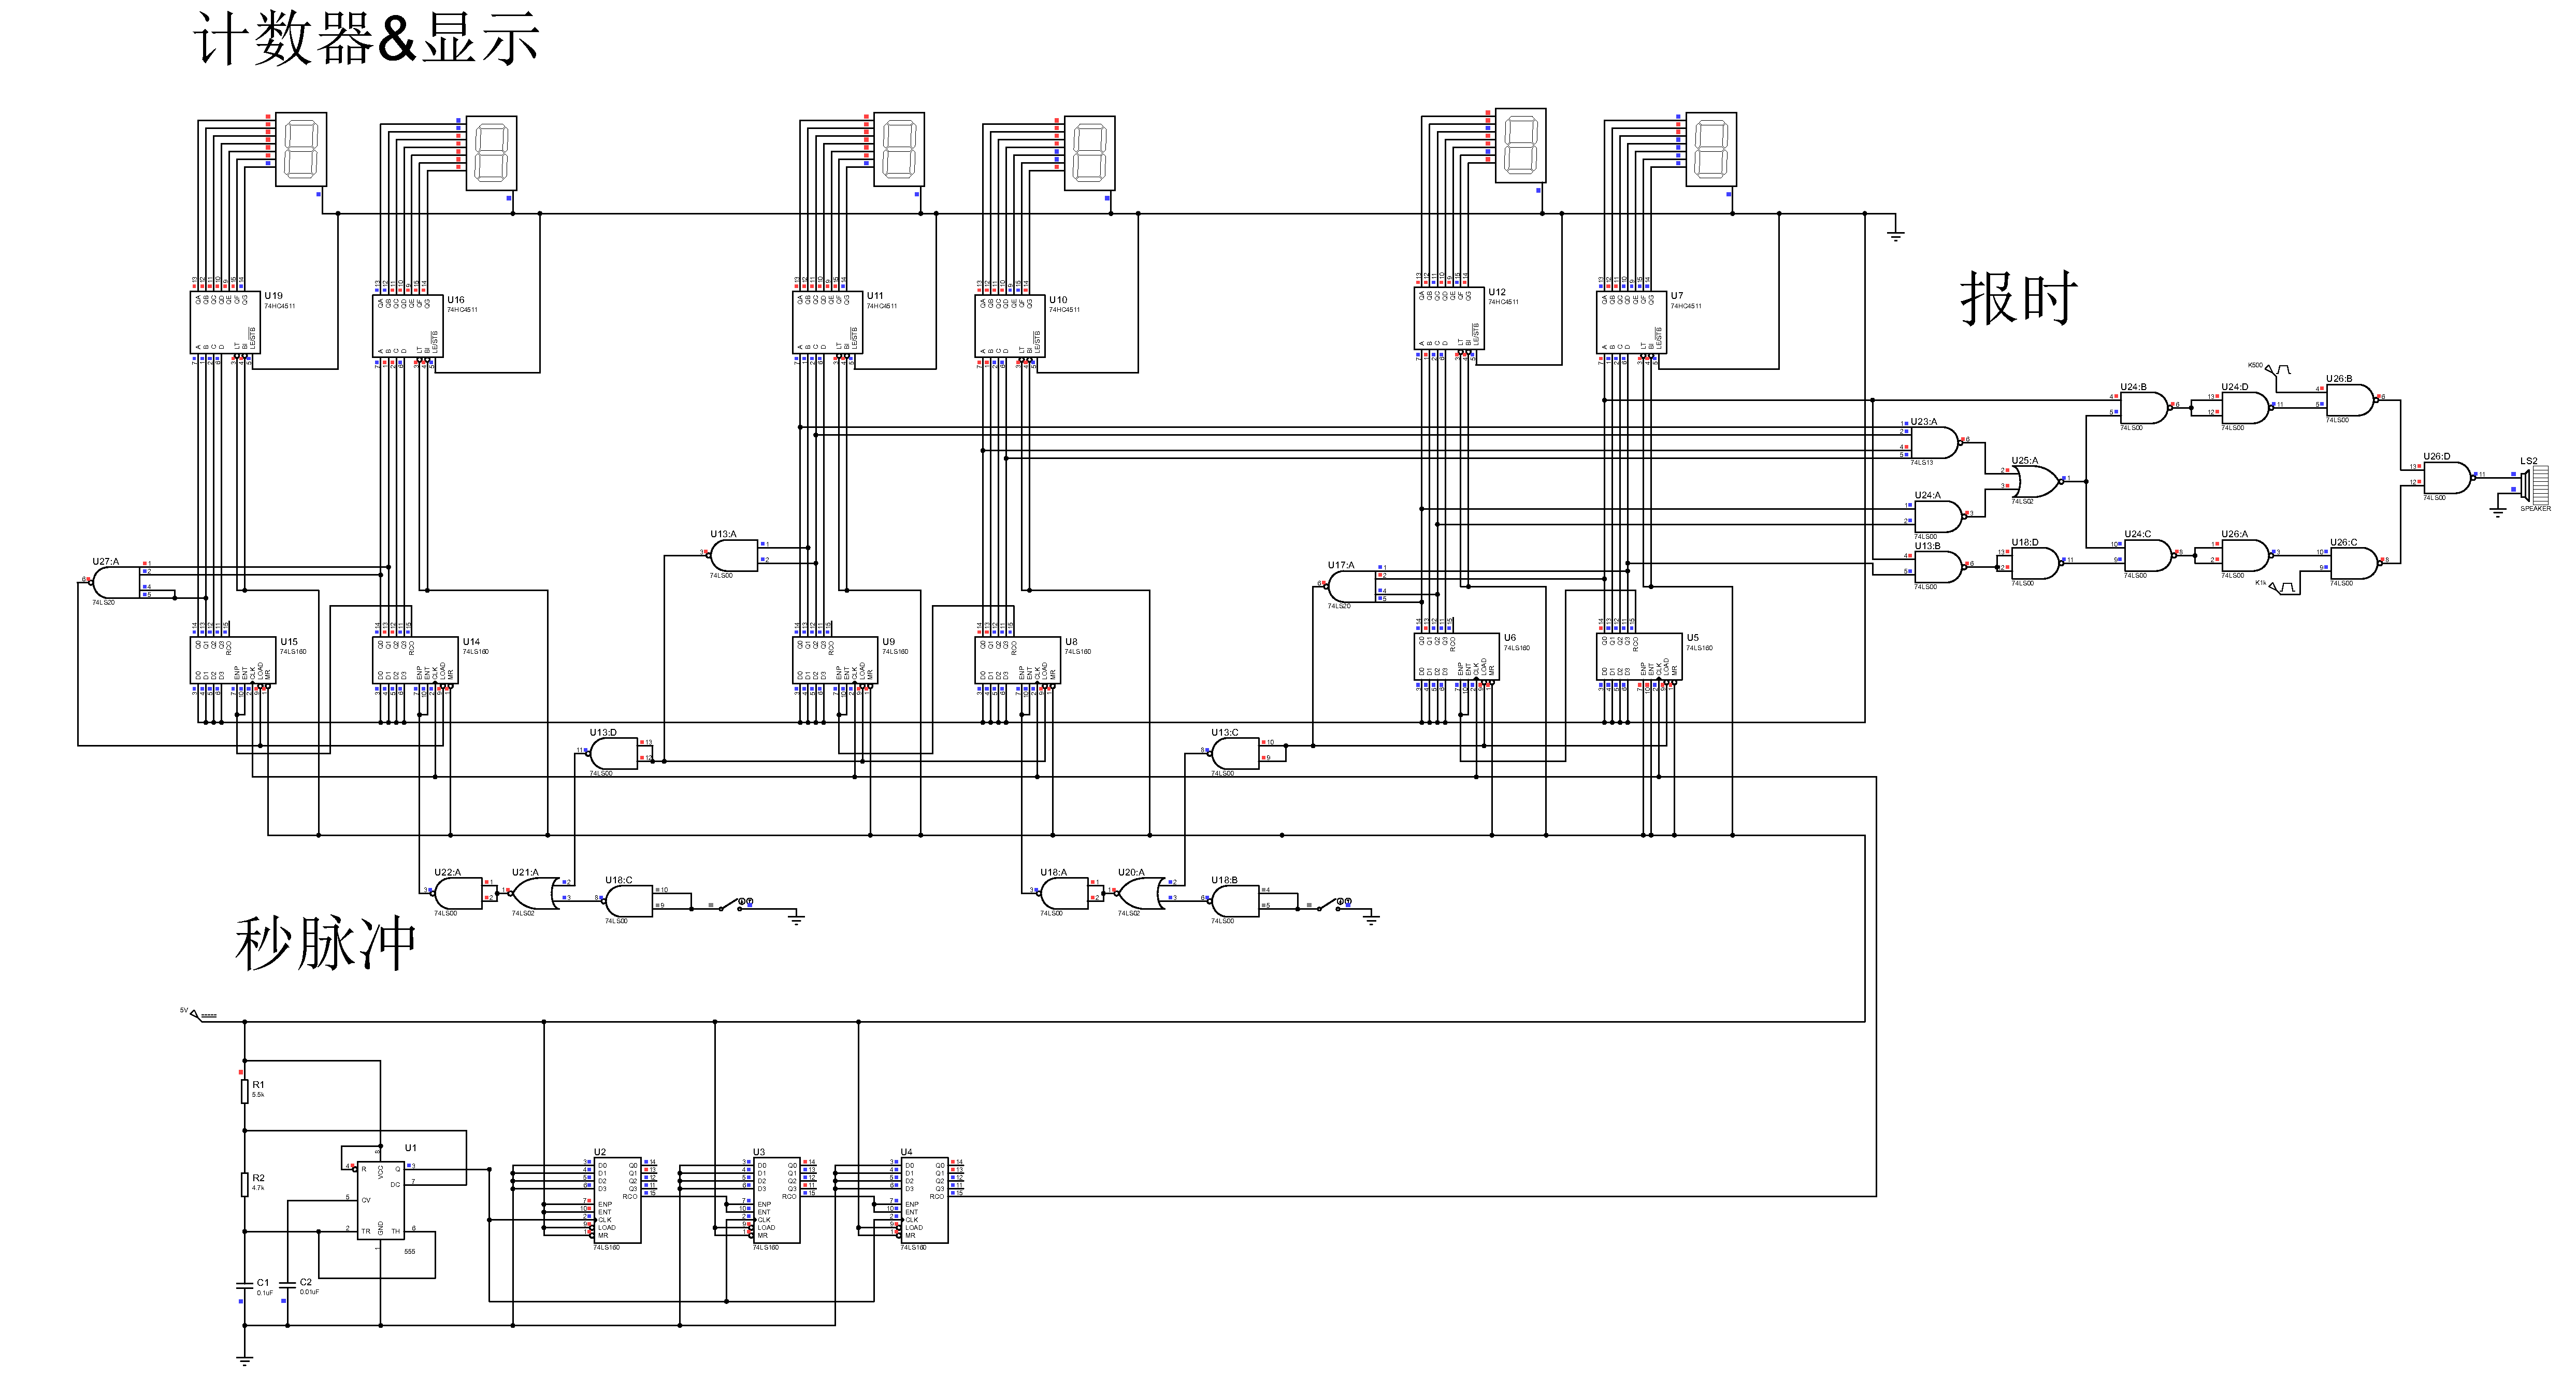
\includegraphics[width=1\textwidth]{pdf/总电路.PDF}
		\caption{总电路图}
	\end{center}
\end{figure}

\subsection{秒脉冲}

\begin{figure}[H]
	\begin{center}
		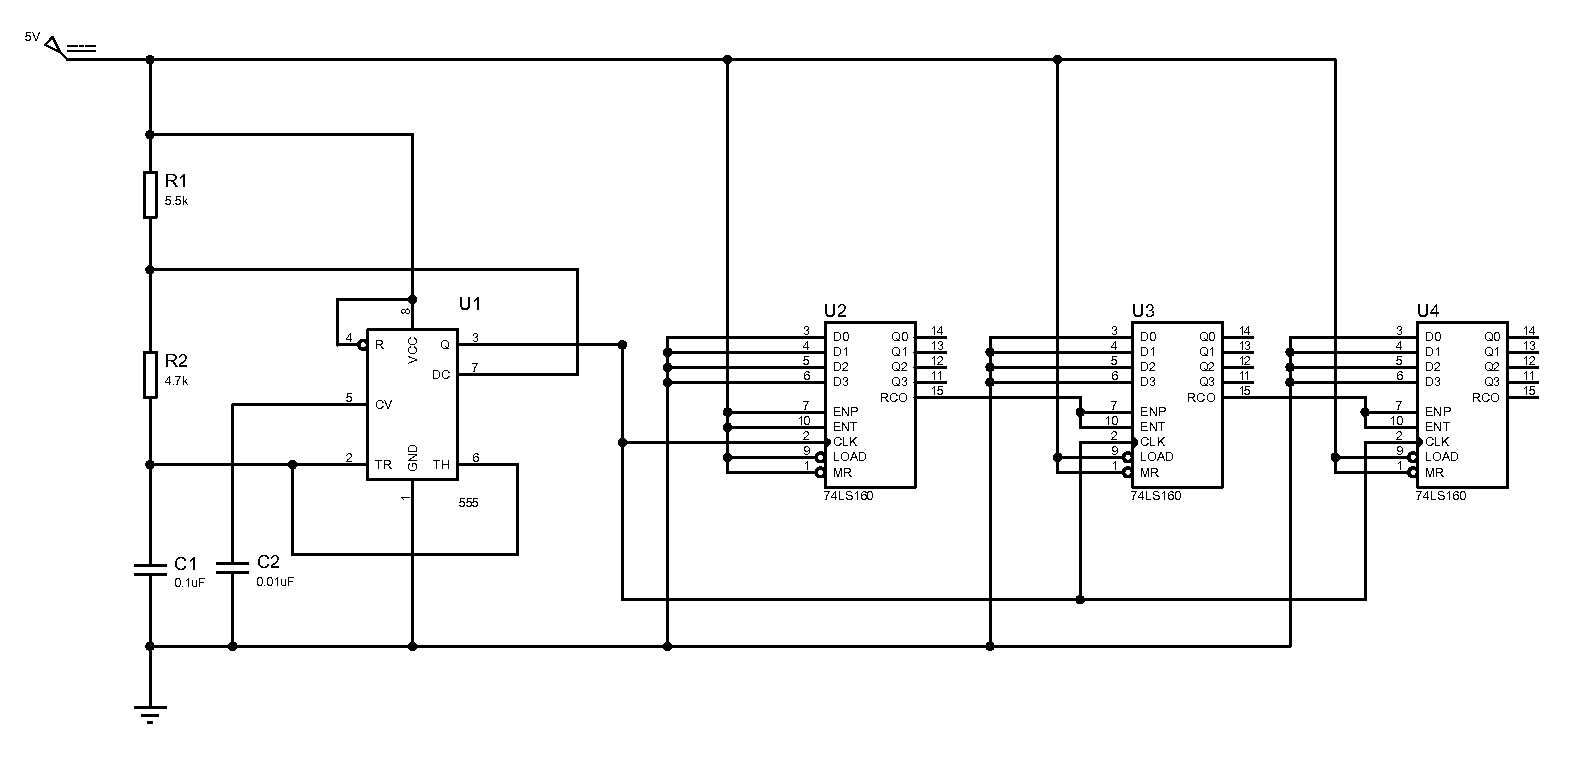
\includegraphics[width=1\textwidth]{pdf/秒脉冲.PDF}
		\caption{秒脉冲电路图\label{ifg:miao}}
	\end{center}
\end{figure}

\paragraph{使用元器件}
\begin{itemize}
	\item 555定时器

		555定时器是一种模、数泥合的中规模集成电路,它使用方便、灵活,应用极为广泛。用它可很方便地组成脉冲的产生、整形、延时和定时电路。
	\item 74LS160

		同步十进制计数器(直接清零),用于快速计数的内部超前进位,由4个主从触发器和用作除2计数器及计数周期长度为除5的3位2进制计数器所用的附加选通所组成。有选通的零复位和置9输入。
\end{itemize}

\paragraph{秒脉冲}由多谐振荡器与滤波器组成。555定时器组成多谐振荡器,振荡出\SI{1}{\kilo\hertz}的脉冲信号,之后由74LS160组成的分频器分别分成\SI{100}{\hertz}、\SI{10}{\hertz}、\SI{1}{\hertz}。最后取\SI{1}{\hertz}作为时钟的脉冲信号。

\paragraph{多谐振荡器-原理}

555定时器接通电源后,电容$C$被充电,当$v_c$上升至$\frac{2 V_{cc}}{3}$时,使$v_0$为低电平,同时$T$导通,此时电容$C$通过$R_2$和$T$放电,$v_c$下降。当$v_c$下降到$\frac{V_{cc}}{3}$时,$v_0$翻转为高电平。如此往复。所以振荡频率为

$$f = \frac{1}{t_{pL} + t_{pH}} \approx \frac{1.43}{(R_1 + 2R_2)C}$$

故选择$R1 = 5.5\si{\kilo}, R2 = 4.7\si{\kilo}, C1 = \SI{0.1}{\mu\farad}, C2=\SI{0.01}{\mu\farad}$

\paragraph{分频器-原理}

74LS160为异步清零同步置数的十进制计数器,将振荡器发出的\SI{1}{\kilo\hertz}脉冲接至CP端,计时器累计到进位时在RCO端输出脉冲信号,实现了十分频。故三片74LS160即可将\SI{1}{\kilo\hertz}的输入型号转化为\SI{1}{\hertz}信号,且第一片的Q0可输出\SI{500}{\hertz}信号。


\begin{table}[H]
	\begin{center}
		\begin{tabular}{|l|l|l|l|l|}
			\hline
			*SR & PE & CET & CEP & 工作模式                   \\ \hline
			L   & X  & X   & X   & RESET (Clear)清零        \\ \hline
			H   & L  & X   & X   & LOAD (Pn  Qn)置数        \\ \hline
			H   & H  & H   & H   & COUNT (Increment)计数    \\ \hline
			H   & H  & L   & X   & NO CHANGE (Hold)保持(不变) \\ \hline
			H   & H  & X   & L   & NO CHANGE (Hold)保持(不变) \\ \hline
		\end{tabular}
		\caption{74LS160真值表}
	\end{center}
\end{table}

\subsection{60进制计数器}

\begin{figure}[H]
	\begin{center}
		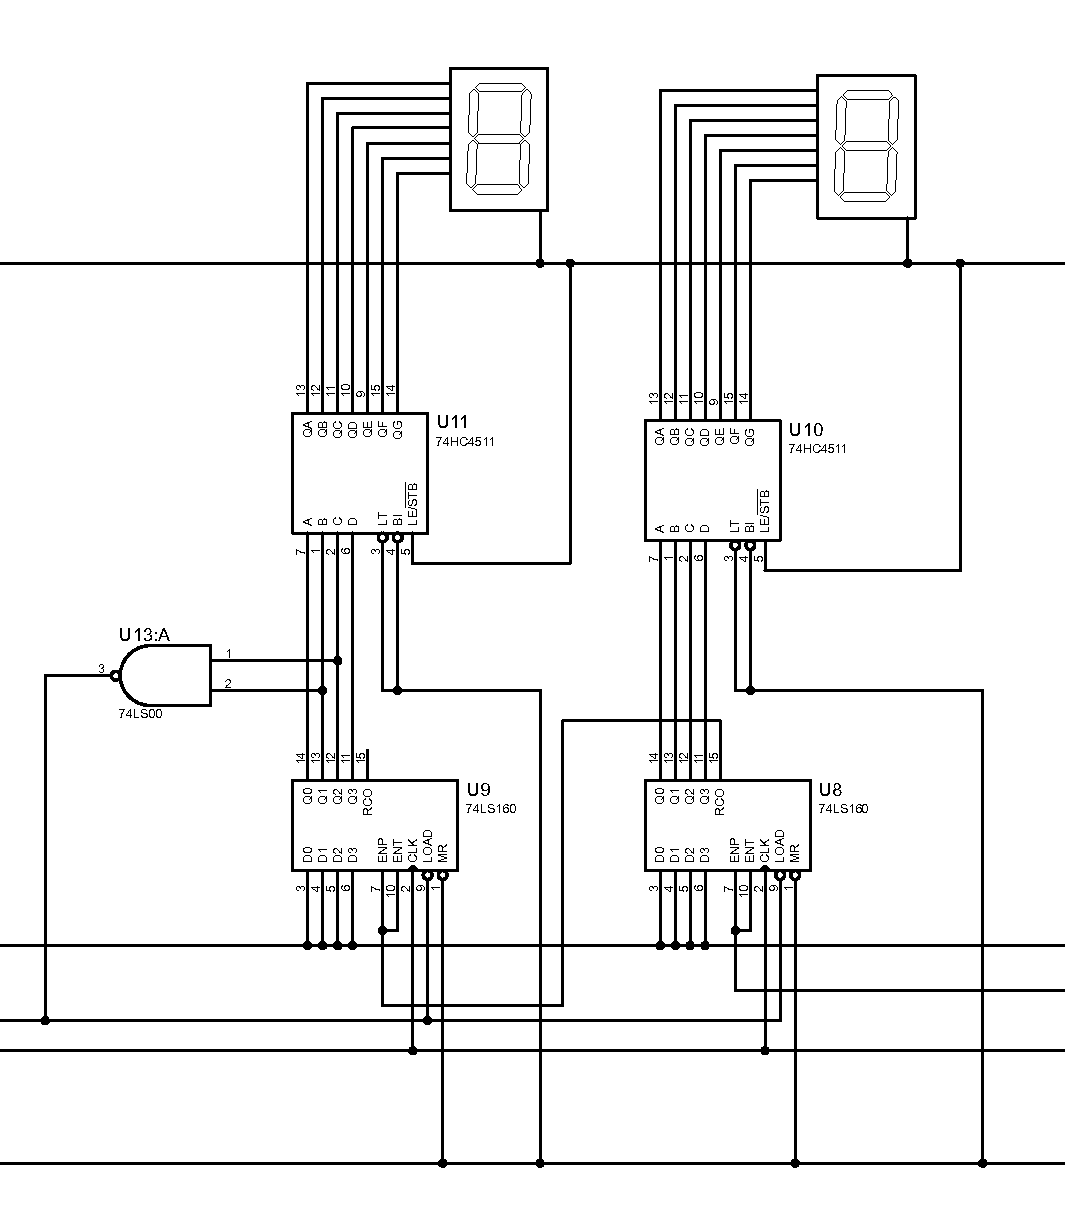
\includegraphics[width=0.5\textwidth]{pdf/计数器-60进制.PDF}
		\caption{60进制计数器\label{ifg:count60}}
	\end{center}
\end{figure}

\paragraph{使用元器件}
\begin{itemize}
	\item 74HC4511:BCD-To-7 Segment 译码器
	\item 7段共阴极数码管
	\item 74LS160:异步清零同步置数的十进制计数器
	\item 74LS00:与非门
\end{itemize}

\paragraph{原理}

通过秒脉冲将\SI{1}{\hertz}脉冲接至2块74LS160CP端,之后将个位的RCO端接至十位的使能端,当个位进位时,十位进行计数。再通过与非门输入十位的Q1,Q2端,输出至两位的LOAD端。实现同步清零。

\subsection{24进制计数器}

\begin{figure}[H]
	\begin{center}
		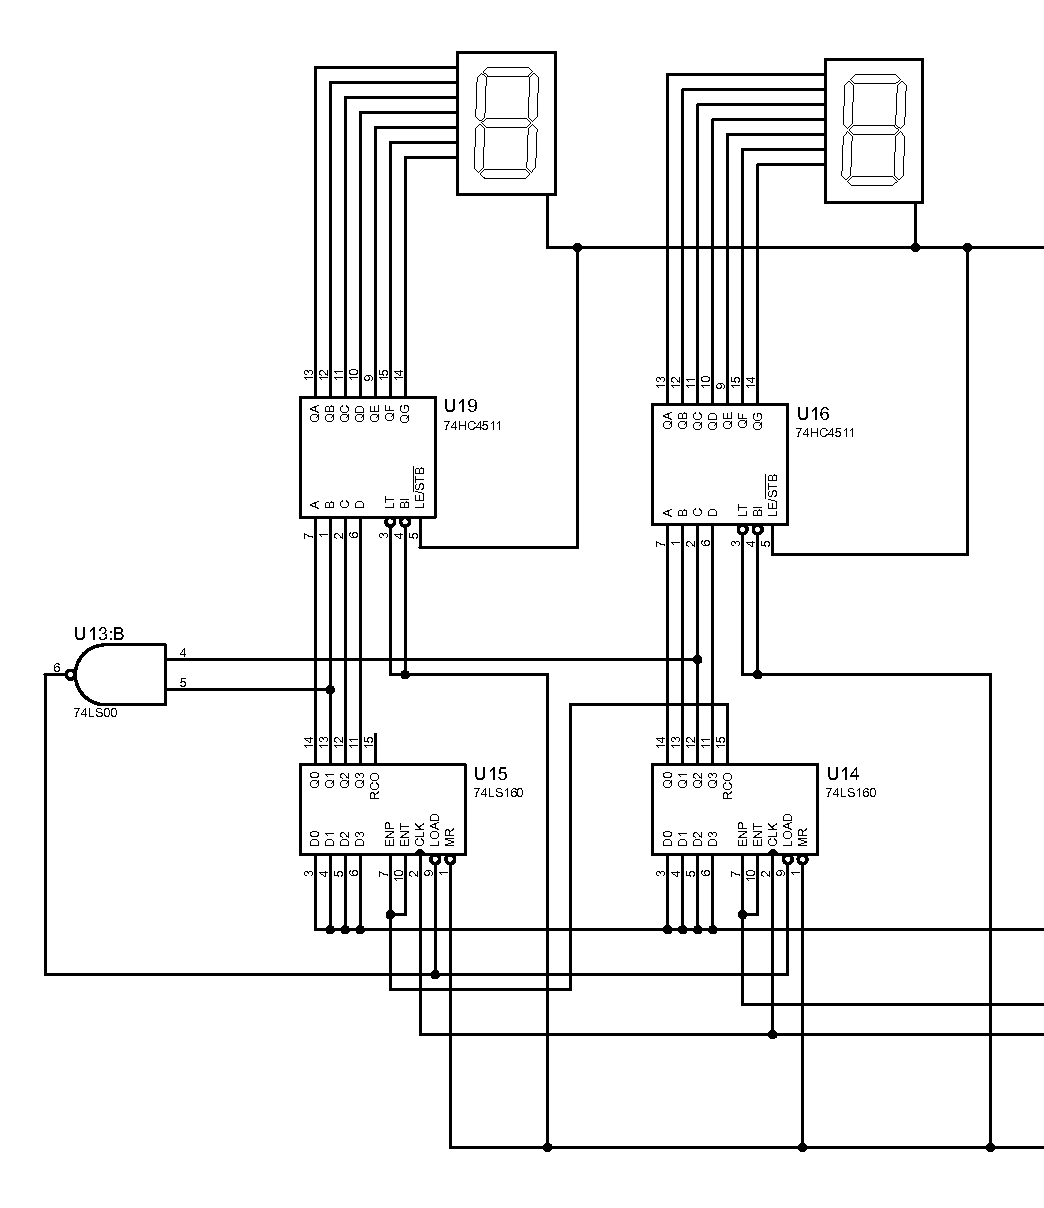
\includegraphics[width=0.5\textwidth]{pdf/计数器-24进制.PDF}
		\caption{24进制计数器\label{ifg:count24}}
	\end{center}
\end{figure}

\paragraph{使用元器件}

\begin{itemize}
	\item 74HC4511:BCD-To-7 Segment 译码器
	\item 7段共阴极数码管
	\item 74LS160:异步清零同步置数的十进制计数器
	\item 74LS00:与非门
\end{itemize}


\paragraph{原理}

通过秒脉冲将\SI{1}{\hertz}脉冲接至2块74LS160CP端,之后将个位的RCO端接至十位的使能端,当个位进位时,十位进行计数。再通过与非门输入十位的Q2与个位的Q3端,输出至两位的LOAD端。实现同步清零。


\subsection{报时电路}

\begin{figure}[H]
	\begin{center}
		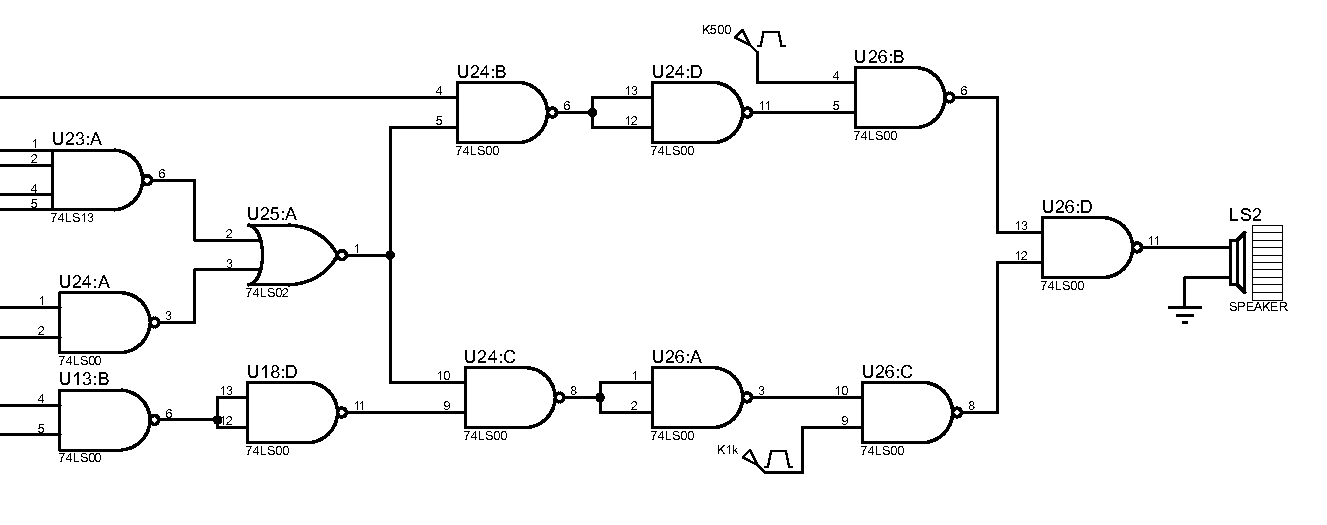
\includegraphics[width=1\textwidth]{pdf/报时电路.PDF}
		\caption{报时电路\label{ifg:speak}}
	\end{center}
\end{figure}

\paragraph{使用元器件}

\begin{itemize}
	\item 74LS00
	\item 74LS13
	\item 74LS02
\end{itemize}

\paragraph{效果}

整点报时电路每小时最后10秒钟,前四声响\SI{500}{\hertz}声音,最后一声响\SI{1}{\kilo\hertz};当秒计数器的个位为1、3、5、7、9时,扬声器振动发声。

\paragraph{原理}
当计数器统计为59时50分时开始处理报时,所以将小时位的十位Q0、十位Q2,个位Q0、个位Q3端连接在同一个与非门中,如\figref{ifg:speak}中U23:A元件,将分钟位十位Q0、十位Q2连接在同一个与非门中,如\figref{ifg:speak}中U24:A元件。当这些位全部为高电平时U25:A元件将输出高电平。
因为我们要处理秒计数器的个位为1、3、5、7、9的情况,我们发现这些位的Q0位都为高电平,故我们只需要取Q0端即可,当Q0端为高电平,并且U25:A元件也为高电平,即可播放声音。不过需要注意在当计数器统计在9位时,要播放\SI{1}{\kilo\hertz}的声音,所以专门将秒计数器的个位Q3位接出来,与U25:A组成一个与非门,并且与\SI{1}{\kilo\hertz}连在一起触发扬声器。

\subsection{快速校时电路}

\begin{figure}[H]
	\begin{center}
		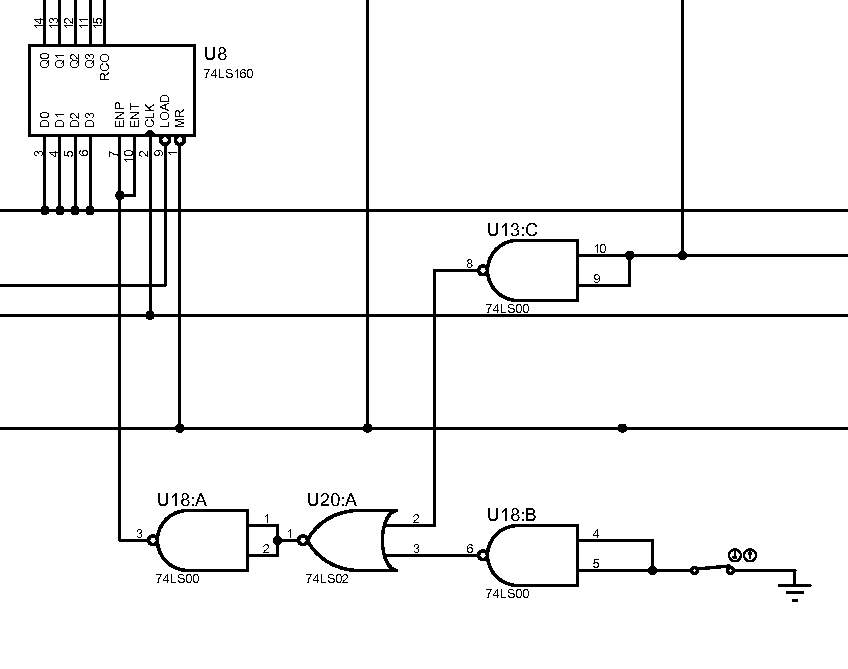
\includegraphics[width=1\textwidth]{pdf/自动校时电路.PDF}
		\caption{自动校时电路\label{ifg:config}}
	\end{center}
\end{figure}

\paragraph{使用元器件}

\begin{itemize}
	\item 74LS00
	\item 74LS02
	\item 开关
\end{itemize}

\paragraph{原理}

74LS00为TTL门,开关断开时输入高电平,开关闭合时输入低电平。根据相应逻辑关系,开关断开时可根据时钟脉冲快速调整时钟分钟,开关闭合时则正常计数。

\section{元器件清单}

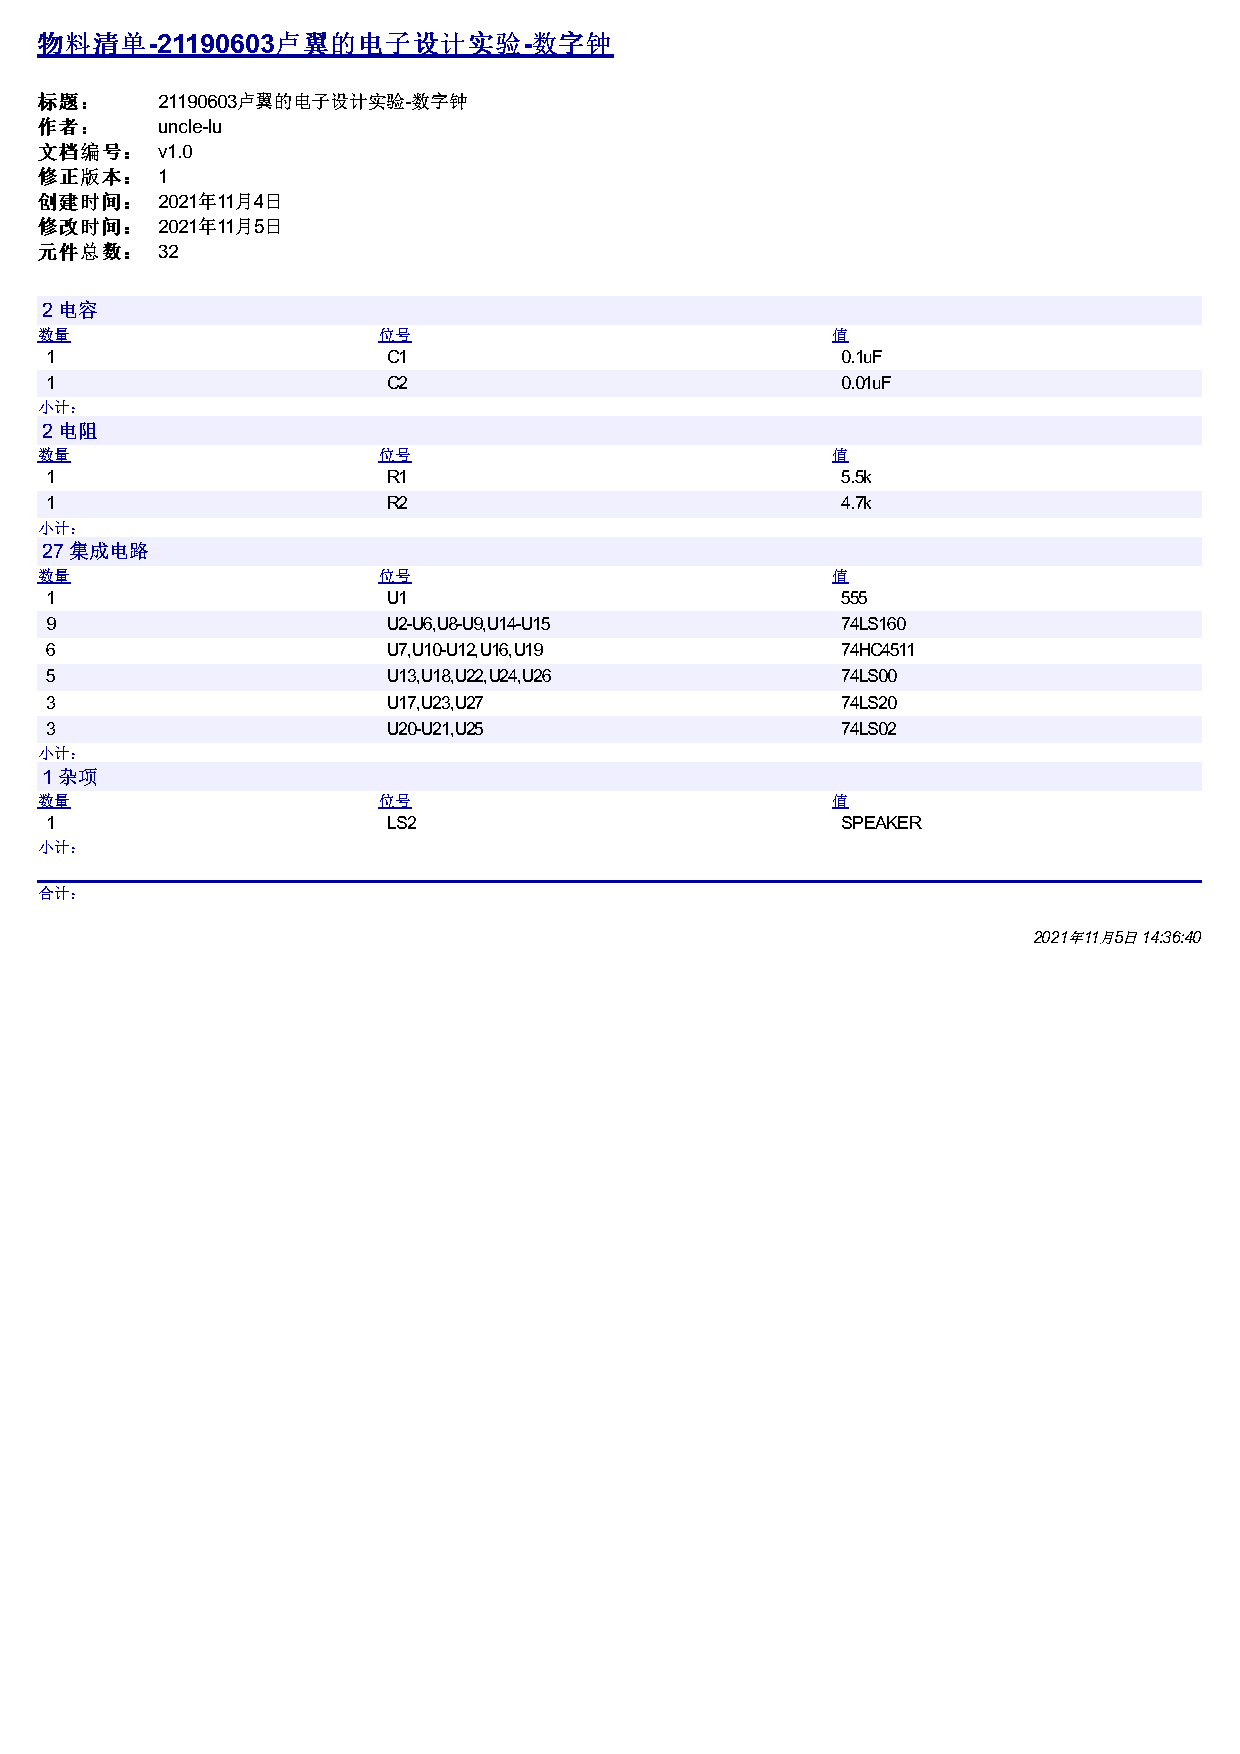
\includepdf{pdf/物料清单.pdf}

\section{实验操作问题}

\paragraph{电源线路连接}

由于面包板的结构,各单元面包板间需要采用导线连接方式保证电路的导通,最初设计采用两组杜邦线分别供给上下两块区域的电源,在实际使用过程中,两组杜邦线增加了接线错误率,同时由于杜邦线本身不能与面包板空隙紧密契合,容易发生脱落。出于实际考量,最后我们将面包板上所有供电线路用普通导线连接,使用一组杜邦线为整个电路供电;二是在设计中,我们采用一行全为地线/+5V供电的设计,然而在实际接线中,发生了两种线路接反的问题,最后通过查线的方式解决了该问题;三是在连接喇叭测试时,误拔了电路的地线,导致\SI{1}{\hertz}脉冲信号消失,通过耐心寻找问题,逐模块检查,最终排除问题。


\paragraph{计数器模块}
本次课程设计中计数器模块是问题相对较多的模块,一方面是由于计数器模块本身连线难度相对较大,较为复杂,一方面是由于该模块是整个数字钟课程设计的核心模块,数字钟相关一系列功能的实现都与其相关,其他模块的故障往往对其也会产生影响。在设计中计数器模块主要产生以下几个问题。
首先是导线的错误连接,导线的错误连接常常发生在初次连接与调试时反复插线时,前者的错误归功于清晰的仿真电路图,错误发生较少,易于检查;后者则相对难以查出,需要对实际电路与原理的清晰认识。
其次是芯片的选择,同型号不同集成电路结构的芯片的负载能力不同,本次设计过程中出现了下一级芯片接收不到上一级进位信号,而进位信号实际存在的问题,分析问题,原因在于上一级的芯片负载能力较弱,无法满足下一级输入信号的进位要求,实验过程中曾尝试使用相同的芯片,结果仍然出现了问题,最终通过逐级更换芯片的方式解决问题。

\paragraph{导线选择}

课程设计实验最初实际接线时,采用普通导线剥线紧贴面包板的方式接线,该方法的好处在于接线清晰明了,弊端在于费时费力,同时对距离较远的两点连接尤为不便,因而在完成主要模块的接线后,整点报时与闹钟模块使用杜邦线接线,加快进度的同时,杜邦线连接门电路可以更好的体现逻辑关系。

\paragraph{仿真与实际接线的差异}

仿真中整点报时电路蜂鸣器输出四低一高的声音信号使用了三极管放大电路,但是实际接线中发现无需三极管放大电路也可以正常输出声音信号,故实际接线可以简化操作。
仿真中多谐振荡器产生的方波信号经过分频器得到的1Hz信号无法直接测出频率判断是否符合要求,实际操作中可以先使用数字示波器观察555芯片输出的信号并通过调节滑动变阻器时期频率为\SI{1}{\kilo\hertz},分频器输出的\SI{1}{\hertz}信号可以通过灯泡大致判断是否符合要求。


\section{心得体会}

本次课程设计在与同伴的通力合作下,顺利完成。期间虽然遇到了一些问题,但是最终都得到了解决。

本次课程设计,主要有两点收获。一是让我认识到仿真的重要性,在本次实验中,只要仿真没有问题,按照仿真电路图接线都可以达到预期效果,详尽合理的前期仿真是实际搭接电路成功的重要保障;二是提高了实际接线与分析实际问题的能力,在实验设计过程中出现了接线错误、芯片选择不合理、线路设计不合理等问题,通过结合专业知识与现实条件,最终解决了问题。

\section{参考文献}

\begin{enumerate}
	\item 康华光;电子技术基础数字部分;华中科技大学电子技术课程组编;第六版;北京高等教育出版社;2014.19
	\item 74LS192、74LS160、74LS00、74LS02、74LS20、74LS86、NE555数据手册
	\item TKD-4型电子设计综合实验箱使用手册
\end{enumerate}



\end{document}
